\documentclass[xcolor=dvipsnames]{beamer}

\graphicspath{ {../Includes/} }

\usetheme{Copenhagen}

\newcommand\Fontvi{\fontsize{7}{10}\selectfont}

\title{A Farewell to Structural Rigidity}
\subtitle{Evolving the Starting State of Autoencoders}
\author[Ross \and Brant \and Roessler]{Christopher Ross \and Jonathan Brant \and Zak Roessler}

\begin{document}

	\begin{frame}
		\titlepage
	\end{frame}
	
	\section{Introduction}
	\begin{frame}{Introduction}	
		\begin{itemize}
			\item Image Processing/Classification
			\begin{enumerate}
				\item Each pixel is a separate input
				\item ANN inputs grows exponentially as resolution increases
				\item Method of dimensionality reduction needed
			\end{enumerate}			
			\item Autoencoders learns compressed representation
			
			\item Traditionally, autoencoder hidden layer topology has been hand-crafted
			
			\item Our approach evolves autoencoder structure that can then be optimized			
			\begin{enumerate}
				\item Hidden layer of autoencoders evolved (using HyperNEAT)
				\item Backpropagation optimizes evolved autoencoder
			\end{enumerate}
		\end{itemize}
	\end{frame}
	
	\section{Background}	
	\begin{frame}{Autoencoders}	
		\begin{columns}[T]
			\begin{column}{.5\textwidth}
				\begin{itemize}
					\item Autoencoders attempt to extract most salient features from visible layer	
					\item Typical layers include:
					\begin{enumerate}\Fontvi
						\item Input (visible) layer where uncompressed features are received
						\item Hidden layer where compressed features are stored
						\item Output layer where reconstruction error is calculated
					\end{enumerate}
					\item Most often trained using backpropagation with the intent of minimizing reconstruction error
				\end{itemize}
			\end{column}
	
			\begin{column}{.5\textwidth}
				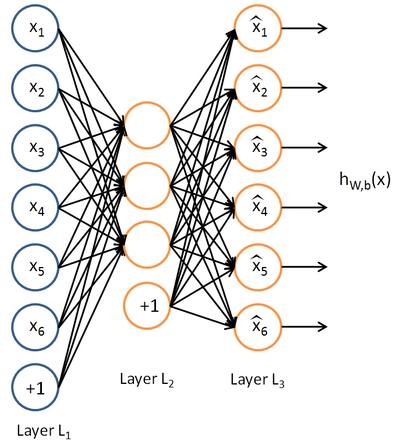
\includegraphics[width=\textwidth]{ExampleAutoencoder}
			\end{column}
		\end{columns}
	\end{frame}
	
	\begin{frame}{HyperNEAT}
		\begin{columns}[T]
			\begin{column}{.5\textwidth}
				\begin{itemize}
					\item Indirect encoding of HyperNEAT through CPPNs substantially reduces search space
					\begin{enumerate}\Fontvi
						\item We're no longer looking at each pixel individually
					\end{enumerate}
					\item Substrate configuration hand-designed to capture domain geometry
					\begin{enumerate}\Fontvi
						\item State-space sandwich substrate ideal for visual mapping
					\end{enumerate}
					\item Ability to scale with little-to-no loss of function ideal for image processing at varying resolutions
				\end{itemize}
			\end{column}
			\begin{column}{.5\textwidth}
				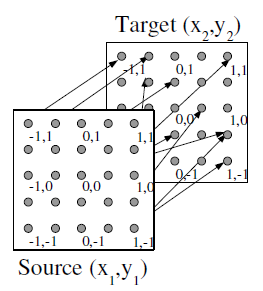
\includegraphics[width=\textwidth]{StateSpaceSandwichSubstrate}
			\end{column}
		\end{columns}			
	\end{frame}
	
	\section{Approach}
	\begin{frame}{Evolution of Autoencoders}
		\begin{itemize}
			\item Two-phase process:
			\begin{enumerate}
				\item HyperNEAT evolves initial autoencoder
				\item Backpropagation fine tunes autoencoder weights
			\end{enumerate}
			
			\bigskip
			
			\item Results will be analyzed:
			\begin{enumerate}
				\item Quantitatively - reduction of reconstruction error
				\item Qualitatively - how closely does reconstructed image resemble the original
			\end{enumerate}
		\end{itemize}				
	\end{frame}
	
	\begin{frame}{Substrate Configuration}
		\begin{columns}[T]
			\begin{column}{.5\textwidth}
				\begin{itemize}
					\item Three-tiered state-space sandwich substrate
					\begin{enumerate}
						\item Input sheet - all points in 2-dimensional image (size varies based on image resolution)
						\item Hidden sheet - compressed feature vector
						\item Output sheet - reconstructed image at original resolution
					\end{enumerate}
				\end{itemize}
			\end{column}
			\begin{column}{.5\textwidth}
				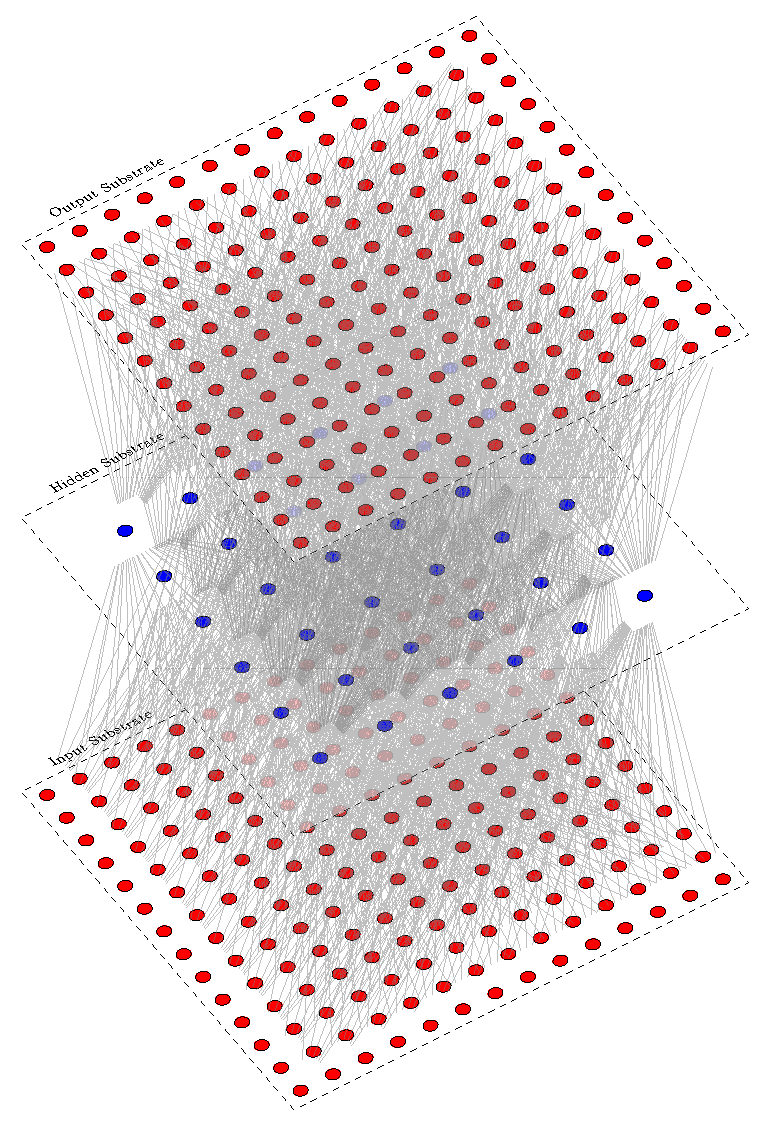
\includegraphics[width=\textwidth,height=0.8\textheight,keepaspectratio]{SubstrateConfiguration/AutoencoderSubstrate}
			\end{column}
		\end{columns}	
	\end{frame}
	
	\begin{frame}{Minimal CPPN}
		\begin{itemize}
			\item CPPN inputs are cartesian coordinates between source and target sheet
			\begin{itemize}\Fontvi
				\item $X_1$ and $Y_1$ is point on source sheet
				\item $X_2$ and $Y_2$ is point on target sheet
			\end{itemize}
			\item CPPN queries the substrate twice:
			\begin{itemize}\Fontvi
				\item Once for connection weight and bias weight between input and hidden sheet
				\item Once for connection weight and bias weight between hidden and output sheet
			\end{itemize}
		\end{itemize}
		\begin{center}
			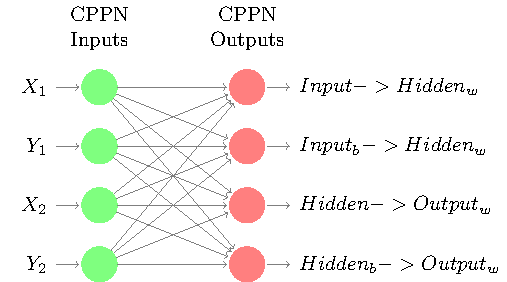
\includegraphics[width=\textwidth,height=0.4\textheight,keepaspectratio]{MinimalCppn/MinimalCppn}
		\end{center}
	\end{frame}
	
	\section{Discussion}
	\begin{frame}{Current State}
		\begin{itemize}
			\item Standard NEAT initially attempted
			\begin{itemize}
				\item Slow evolution due to massive search space
				\item Qualitatively poor image reconstruction
				\item Reconstruction reached 90\% accuracy, but only because most pixels were black
			\end{itemize}
			\item HyperNEAT results?
		\end{itemize}
	\end{frame}

\end{document}